\documentclass[preprint,12pt,authoryear]{elsarticle}
\usepackage{amsmath,amssymb}
\usepackage{graphicx}
\usepackage{booktabs}
\emergencystretch=2em
\usepackage{array}
\usepackage{rotating}
\usepackage{hyperref}
\usepackage{xcolor}
\graphicspath{{../../results/figures/}}
\newcommand{\dirMaxDSRDev}{0.58}
\newcommand{\dirMeanICDev}{-0.004}
\newcommand{\dirMaxDSRCon}{0.46}
\newcommand{\dirMeanICCon}{0.003}


\journal{International Journal of Forecasting}

\begin{document}
\begin{frontmatter}

\title{Is the predictability in risk or in direction? A pre-registered evaluation of
regime-conditioned analogue forecasting in financial markets}

\author[cse]{Manas Ganesh Dasari\corref{cor1}}
\ead{bl.sc.u4cse24229@bl.students.amrita.edu}
\author[cse]{Vishal KVS}
\author[math]{K. N. Meera}
\cortext[cor1]{Corresponding author}
\affiliation[cse]{organization={Department of Computer Science and Engineering, Amrita School of Computing, Amrita Vishwa Vidyapeetham},
  city={Bengaluru}, country={India}}
\affiliation[math]{organization={Department of Mathematics, Amrita School of Computing, Amrita Vishwa Vidyapeetham},
  city={Bengaluru}, country={India}}

\begin{abstract}
Analogue (nearest-neighbour) forecasting is popular in trading because each forecast is backed by
concrete historical episodes, but it is easy to evaluate wrongly. We build a leakage-safe analogue
engine---with an exclusion zone that keeps analogue outcomes independent, a Markov mixture over
volatility regimes and labels produced by the same trade simulator that executes the
strategy---and ask where analogue information is predictive. After a development study on nine
assets, we pre-registered eight hypotheses and tested them on fifteen new cryptocurrencies, equity
indices, commodities and currencies. All eight replicated. Analogues carry no information about the
direction of prices: information coefficients are within $\pm0.06$ and no strategy survives a
deflated-Sharpe test. They are informative about risk: combined with HAR they are statistically
indistinguishable from HAR and stay in the model confidence set for 23 of 25 confirmatory series,
while gradient-boosted trees given the same inputs are markedly worse; kernel weighting improves the analogue
forecaster by 5\%; analogue-conditioned Value-at-Risk is as well calibrated as filtered historical
simulation; and volatility-managed exposure reduced the maximum drawdown for all 24 assets without
raising Sharpe ratios. A static Poisson crash gate of the kind used in trading software is worse
than a constant forecast in 31 of 40 series, and a Hawkes process improves on it but not on a logistic model of
current volatility. Code, data scripts and the pre-registration are public.
\end{abstract}


\begin{keyword}
Analogue forecasting \sep Nearest neighbours \sep Volatility forecasting \sep Value-at-Risk \sep
Hawkes process \sep Pre-registration \sep Model confidence set
\end{keyword}
\end{frontmatter}

%% ==================================================================
\section{Introduction}

Forecasting by analogy is one of the oldest ideas in prediction. \citet{lorenz1969} asked how
well the atmosphere could be forecast by finding past states that resemble today's and
following what happened next; \citet{farmer1987} turned the idea into nearest-neighbour
prediction of chaotic time series. In finance, analogue (nearest-neighbour) methods have been
applied to exchange rates \citep{fernandez1999} and are now common in retail trading software,
where their appeal is interpretability: each forecast rests on a list of concrete historical
episodes that a user can inspect, in contrast to the opaque internal states of deep networks.

This paper began as an attempt to publish such a system: a trading engine that matched the
current 20-bar return against history with a one-dimensional $k$-nearest-neighbour rule,
adjusted the resulting win rate with a two-state Markov chain on volatility, suspended trading
when a Poisson estimate of the probability of a large price jump exceeded a threshold, and sized
positions with a fractional Kelly criterion \citep{kelly1956}. Its in-sample backtests on Bitcoin
and gold looked favourable. Rebuilding it for a rigorous evaluation changed the question.
Analogue methods are easy to evaluate wrongly: an analogue whose outcome window has not closed
leaks the future; adjacent bars have near-identical features, so the $k$ nearest analogues are
often one episode counted $k$ times; and trying many configurations and reporting the best
inflates performance \citep{bailey2014,harvey2016}. Once these problems are removed, the natural
question is not whether one configuration is profitable but \emph{where}, if anywhere, analogue
information is predictive.

We answer that question with a leakage-safe analogue engine and a two-stage design. A
\emph{development} study on nine assets (three hourly cryptocurrencies, six daily equity, bond,
gold and currency series) was used for all model building. Its findings were then turned into
eight hypotheses and \emph{pre-registered}---the hypotheses, models, asset list and analysis code
were committed to a public repository and tagged before any data for the confirmatory assets was
downloaded---and tested on fifteen new assets. Pre-registration is standard in experimental
sciences \citep{nosek2018} and has been advocated for empirical finance \citep{harvey2017}, but it
remains rare in forecasting studies.

The analogue engine is used for four targets: the direction of a trade (the original use), the
realised variance of returns over the next $h$ bars, the probability of a large jump, and the
one-day return distribution (Value-at-Risk and Expected Shortfall). Each is compared with
standard benchmarks under a walk-forward protocol: HAR \citep{corsi2009} and GARCH
\citep{bollerslev1986} for volatility, Hawkes processes \citep{hawkes1971} for jumps, filtered
historical simulation \citep{baroneadesi1999} and GARCH-$t$ for tail risk, and gradient-boosted
trees \citep{friedman2001} as a flexible machine-learning comparator.

The closest antecedent is \citet{andrada2016}, who showed in this journal that nearest-neighbour
forecasts of S\&P 100 realised variance, alone and combined with long-memory models, add value
mainly in economic rather than statistical terms. We extend that question from one index to 24
assets in five asset classes, from volatility to direction, jumps and Value-at-Risk, and from a
retrospective study to a pre-registered, prospective test.

Our contributions are threefold. First, we provide a pre-registered, multi-asset evaluation of
analogue forecasting across direction and risk, with the model confidence set
\citep{hansen2011}, Diebold--Mariano tests \citep{diebold1995}, the Fissler--Ziegel loss for
VaR/ES \citep{fissler2016,patton2019} and deflated Sharpe ratios \citep{bailey2014}; to our
knowledge it is the first pre-registered study of analogue forecasting in finance. Second, we
introduce design elements that make analogue forecasts statistically meaningful: an exclusion
zone that keeps analogue outcome windows independent, a mixture over volatility regimes weighted
by the Markov forecast of the regime over the horizon, and labels produced by the same trade
simulator that executes the strategy. Third, we release the engine and every script as
open-source software, so that each table in this paper is reproduced by one command.

The results are summarised in Section~\ref{sec:results}. In brief, analogue methods carry no
information about direction, but they produce risk forecasts that are competitive with the best
standard models, with tail forecasts as well calibrated as filtered historical simulation.

%% ==================================================================
\section{Related literature}

\paragraph{Analogue and nearest-neighbour forecasting} After \citet{lorenz1969} and
\citet{farmer1987}, nearest-neighbour predictors were applied to financial series under the
hypothesis that nonlinear deterministic structure could be exploited where linear models fail.
\citet{fernandez1999} found that simultaneous nearest-neighbour predictors improved on random-walk
forecasts of European exchange rates. The weak-form efficient-markets hypothesis \citep{fama1970}
predicts that such directional structure should be absent or small relative to trading costs.
For risk, \citet{andrada2016} forecast S\&P 100 realised variance with nearest neighbours and
combined them with long-memory models; the combinations were not uniformly more accurate, but
nearest-neighbour forecasts earned higher risk-adjusted returns in an options-trading exercise
during turbulent periods. Similarity-based forecasting has also been formalised for macroeconomic
series \citep{dendramis2020}, and similarity between past shock episodes has been used to correct
GARCH forecasts after news shocks \citep{lundquist2024}.
Kernel regression \citep{nadaraya1964,watson1964} is the smooth counterpart of $k$NN averaging and
appears here as a variant of the engine.

\paragraph{Volatility forecasting} Volatility clustering makes risk far more predictable than
returns. GARCH(1,1) \citep{bollerslev1986} is hard to beat in large comparisons
\citep{hansen2005}; the heterogeneous autoregressive (HAR) model \citep{corsi2009} captures long
memory with three averages of past variance, and in a recent comparison across 1,445 stocks no
machine-learning model beat it once its estimation window and re-estimation frequency were chosen
carefully \citep{chassot2026}. Comparing volatility forecasts requires loss
functions that are robust to noise in the realised proxy; QLIKE and MSE on the variance scale
are robust in this sense \citep{patton2011}. The model confidence set \citep{hansen2011}
identifies the set of models that cannot be distinguished from the best.

\paragraph{Jumps and self-excitation} Large price moves cluster. Hawkes processes
\citep{hawkes1971} model this through an intensity that jumps after each event and decays; they
are widely used for market microstructure \citep{bacry2015} and for contagion between markets
\citep{aitsahalia2015}. The original system used a static Poisson rate estimated over a long
window, which cannot represent clustering.

\paragraph{Tail-risk forecasting} Filtered historical simulation \citep{baroneadesi1999} rescales
historical standardised residuals by a current volatility forecast. Coverage of VaR forecasts is
assessed with the tests of \citet{kupiec1995} and \citet{christoffersen1998}. Expected Shortfall is
not elicitable on its own but is jointly elicitable with VaR \citep{fissler2016}, and the FZ0 loss
of \citet{patton2019} is the standard tool for comparing (VaR, ES) forecasts.

\paragraph{Economic value and overfitting} Scaling exposure inversely to forecast variance
improves risk-adjusted returns in some samples \citep{moreira2017}, but out-of-sample gains are
fragile \citep{cederburg2020}. Backtests of many configurations must be deflated for multiple
testing \citep{bailey2012,bailey2014,harvey2016}.

%% ==================================================================
\section{Methodology}
\label{sec:method}

\subsection{The analogue engine}
Let $x_t\in\mathbb{R}^m$ be a causal embedding of the state at bar $t$ and $y_j\in\mathbb{R}^p$ a
vector of targets attached to anchor $j$, fully observed at $j+\delta$. At bar $t$ the candidate
set is $\mathcal{C}_t=\{j: j\le t-\delta\}$, so no candidate's outcome extends beyond $t$.
Distances are Euclidean, $d_{tj}=\lVert x_t-x_j\rVert$.

\paragraph{Exclusion zone} Candidates are accepted in increasing distance, but a candidate is
skipped if it lies within $e$ bars of an already accepted analogue. With $e\ge h$ the outcome
windows of accepted analogues do not overlap, so their outcomes are not mechanically
dependent. Without this rule the nearest neighbours of a smooth feature are usually adjacent
bars from one episode. A configuration guard rejects settings in which $2ke$ exceeds a quarter
of the available history, because the greedy rule would then be forced to accept distant,
non-analogous candidates.

\paragraph{Regime mixture} Each bar has a volatility state $s_t\in\{0,1\}$ (ATR above or below its
long moving average, following \citealp{wilder1978}). Analogues are selected separately within
each regime, giving group means $\bar y_0(t)$ and $\bar y_1(t)$. A two-state Markov chain
estimated on past transitions gives the probability $\pi_1(t)$ of being in the high state,
averaged over the next $h$ steps; the forecast is
$\hat y_t = (1-\pi_1)\bar y_0 + \pi_1 \bar y_1$ with standard error
$\big[(1-\pi_1)^2 \hat\sigma_0^2/k_0 + \pi_1^2 \hat\sigma_1^2/k_1\big]^{1/2}$. This replaces the ad hoc
adjustment of the original system, which shrank the analogue win rate toward one half by the
persistence probability, with an application of the law of total probability over regimes
\citep[cf.][]{hamilton1989}.

\paragraph{Kernel variant} Instead of $k$ neighbours, all candidates can be weighted by
$w_{tj}=\exp(-d_{tj}^2/2b^2)$; standard errors then use the \citet{kish1965} effective sample size.

\subsection{Direction model}
The embedding is the last $w=20$ log returns summed into $m$ segments and scaled by the EWMA
volatility at $t$; $m=1$ without scaling is the feature of the original system. The target is
not the sign of a future return but the net R-multiple of the exact trade the strategy would
take at the anchor: entry at the next open, stop $2.5\times$ATR, target $1.5\times$ the stop, exit
after $h=20$ bars, costs deducted. The same simulator executes live signals, so labels and
execution cannot disagree. A long (short) trade is entered when the lower confidence bound
$\hat R - z\,\mathrm{se}$ is positive and exceeds the opposite side's; the fraction of equity risked
is the fractional Kelly quantity $\tfrac12\,\mathrm{E}[R]/\mathrm{E}[R^2]$, capped at 2\%.

\subsection{Volatility model}
The target is $\log \mathrm{RV}_{t,h}$ with $\mathrm{RV}_{t,h}=h^{-1}\sum_{u=1}^{h} r_{t+u}^2$ and
$h=24$ for hourly and $h\in\{5,22\}$ for daily series. The analogue embedding is the \emph{shape}
of recent volatility: the log mean squared return in $m=4$ consecutive segments of $h$ bars, each
relative to a long-run EWMA variance $\bar\sigma^2_t$. The analogues forecast the log ratio of
future variance to $\bar\sigma_t^2$. We also report \emph{Analogue+HAR}, the equal-weight average
of the analogue and HAR log forecasts. Log-scale forecasts are converted to the variance scale
with the mean exponentiated residual of the fitting window.

Benchmarks are EWMA \citep{riskmetrics1996} with half-life chosen by QLIKE on the fitting window
from $\{5,10,20,50,100,200\}$; GARCH(1,1) with variance targeting and its closed-form $h$-step
mean; log-HAR with averages over $(1, 5, 22)$ days or $(1, 24, 168)$ hours; and gradient-boosted
trees (histogram-based, 300 iterations, learning rate 0.05, no tuning) given the union of the HAR
inputs, the analogue embedding, the regime and the long-run level.

\subsection{Tail events}
A raw jump occurs at $t$ when $|r_t|>3\,\bar\sigma_{t-1}$, measured against the long-run rather
than the current volatility so that volatility clustering is not normalised away. The target is
whether at least one jump occurs in the next $h$ bars. Forecasts: the fitting-window base rate;
the static Poisson estimate of the original system, $1-\exp(-\hat\lambda h)$ with $\hat\lambda$ the
jump rate over the last 1,000 bars; an exponential Hawkes process with intensity
$\lambda(t)=\mu+\alpha\beta\sum_{t_i<t}e^{-\beta(t-t_i)}$, fitted by maximum likelihood, giving
$1-\exp\{-\mu h-\alpha S_t(1-e^{-\beta h})\}$ with $S_t$ the decayed event count; a logistic
regression on $\log(\hat\sigma^2_{\mathrm{EWMA},t}/\bar\sigma^2_t)$; and the analogue frequency.

\subsection{Value-at-Risk and Expected Shortfall}
For one-day VaR and ES at $\alpha\in\{1\%,2.5\%,5\%\}$ all models except historical simulation
(HS, 250 days) use the same GARCH(1,1) forecast $\hat\sigma_{t+1}$, isolating the shape of the
innovation distribution: Gaussian (GARCH-N), standardised Student-$t$ with maximum-likelihood
degrees of freedom (GARCH-$t$), the empirical distribution of all past standardised residuals
(FHS), and the weighted empirical distribution of the standardised residuals that followed the
$k$ nearest volatility-shape analogues (Analogue). \emph{Blend} averages the Analogue and FHS
quantiles and shortfalls.

\subsection{Volatility-managed exposure}
A long position is scaled by $\min(\sigma^\ast/\hat\sigma_{t},1)$, where $\sigma^\ast$ is the average
volatility in the calibration period, with no leverage, a rebalancing band of 0.1 and costs of
5\,bp per unit of turnover. A variant additionally sets exposure to zero when the Hawkes jump
probability exceeds its calibration-period 90th percentile, reproducing the ``lock'' of the
original system.

%% ==================================================================
\section{Experimental design}
\label{sec:design}

\paragraph{Data} Hourly spot prices from Binance and daily prices from Yahoo Finance
(Table~\ref{tab:data}). The development set comprises BTC, ETH and PAXG (a gold-backed token)
hourly from 2018 (PAXG from 2020), and the S\&P 500 (from 1927), Nasdaq-100 ETF, gold ETF,
long-Treasury ETF, EUR/USD and NIFTY 50 daily. The confirmatory set, fixed in the
pre-registration, comprises SOL, BNB, XRP, ADA and LTC hourly and DAX, Nikkei 225, FTSE 100, Hang
Seng, Russell 2000 ETF, emerging-markets ETF, silver ETF, oil ETF, GBP/USD and USD/JPY daily.
Daily Yahoo series pass a documented filter that removes isolated bad prints (a move of more
than eight 20-day standard deviations reversed by more than 70\% on the next bar).

\paragraph{Walk-forward protocol} Each series is split into a calibration period (the first 30\%
of bars, and at least the warm-up plus 500 bars) and an out-of-sample period of five consecutive
folds. For each fold, every fitted quantity---EWMA half-life, GARCH, HAR, gradient boosting,
Hawkes and logistic parameters, bias corrections, and the direction model's configuration
chosen from an 18-point grid---uses only data observed before the fold. All results are
out-of-sample.

\paragraph{Statistics} Volatility forecasts are compared with QLIKE, which ranks forecasts
consistently even when the volatility proxy is noisy \citep{patton2011}; the MSE of log variance is
reported for interpretation only, because it lacks that robustness. We use Diebold--Mariano
tests with Newey--West variance at lag $h$ \citep{newey1987}, and the 90\% model confidence set
with the $T_{\max}$ statistic and 1,000 stationary-bootstrap draws \citep{politis1994}. Jump
forecasts use log-loss, Brier score and AUC. VaR/ES forecasts use Kupiec and Christoffersen tests,
tick loss and the FZ0 loss, with a model confidence set on FZ0. Trading results use Sharpe ratios,
drawdowns, the deflated Sharpe ratio for the direction grid, and paired stationary-bootstrap tests
of Sharpe differences.

\paragraph{Pre-registration} After the development study, eight hypotheses
(Table~\ref{tab:hyp}), the confirmatory asset list, an exclusion rule (fewer than 20,000 hourly or
3,000 daily bars), the unchanged model code and the analysis script were committed to the public
repository and tagged \texttt{prereg-v1} before any confirmatory data was downloaded. Tests are
across series; family-wise error over the eight primary endpoints is controlled with Holm's method
\citep{holm1979}. Development-set results are exploratory---some were inspected during model
building---and are never pooled with confirmatory results.

%% Results, discussion and conclusion. Tables are generated by paper/make_tables.py.

\begin{table}[t]
\centering\scriptsize
\caption{Data. Out-of-sample (OOS) bars follow the calibration period (volatility study, $h=24$
hourly, $h=5$ daily).}
\label{tab:data}
\resizebox{\linewidth}{!}{\begin{tabular}{lllllllrr}
\toprule
Set & Series & Ticker & Source & Freq. & Start & End & Bars & OOS bars \\
\midrule
Development & BTC & BTCUSDT & Binance & 1h & 2018-01-01 & 2026-09-30 & 76,544 & 53,581\\
 & ETH & ETHUSDT & Binance & 1h & 2018-01-01 & 2026-09-30 & 76,544 & 53,581\\
 & PAXG & PAXGUSDT & Binance & 1h & 2020-08-28 & 2026-09-30 & 53,354 & 37,348\\
 & S\&P 500 & \textasciicircum{}GSPC & Yahoo & 1d & 1927-12-30 & 2026-09-29 & 24,802 & 17,362\\
 & Nasdaq-100 & QQQ & Yahoo & 1d & 1999-03-10 & 2026-09-28 & 6,931 & 4,852\\
 & Gold & GLD & Yahoo & 1d & 2004-11-18 & 2026-09-28 & 5,498 & 3,849\\
 & Treasuries & TLT & Yahoo & 1d & 2002-07-30 & 2026-09-28 & 6,080 & 4,256\\
 & EUR/USD & EURUSD=X & Yahoo & 1d & 2003-12-01 & 2026-09-28 & 5,920 & 4,144\\
 & NIFTY 50 & \textasciicircum{}NSEI & Yahoo & 1d & 2007-09-17 & 2026-09-29 & 4,670 & 3,115\\
\midrule
Confirmatory & SOL & SOLUSDT & Binance & 1h & 2020-08-11 & 2026-09-30 & 53,775 & 37,643\\
 & BNB & BNBUSDT & Binance & 1h & 2018-01-01 & 2026-09-30 & 76,551 & 53,586\\
 & XRP & XRPUSDT & Binance & 1h & 2018-05-04 & 2026-09-30 & 73,625 & 51,538\\
 & ADA & ADAUSDT & Binance & 1h & 2018-04-17 & 2026-09-30 & 74,037 & 51,826\\
 & LTC & LTCUSDT & Binance & 1h & 2018-01-01 & 2026-09-30 & 76,551 & 53,586\\
 & DAX & \textasciicircum{}GDAXI & Yahoo & 1d & 1987-12-30 & 2026-09-29 & 9,799 & 6,860\\
 & Nikkei 225 & \textasciicircum{}N225 & Yahoo & 1d & 1965-01-05 & 2026-09-28 & 15,174 & 10,622\\
 & FTSE 100 & \textasciicircum{}FTSE & Yahoo & 1d & 1984-01-03 & 2026-09-29 & 10,797 & 7,558\\
 & Hang Seng & \textasciicircum{}HSI & Yahoo & 1d & 1986-12-31 & 2026-09-28 & 9,807 & 6,865\\
 & Russell 2000 & IWM & Yahoo & 1d & 2000-05-26 & 2026-09-29 & 6,624 & 4,637\\
 & Emerging mkts & EEM & Yahoo & 1d & 2003-04-14 & 2026-09-29 & 5,903 & 4,133\\
 & Silver & SLV & Yahoo & 1d & 2006-04-28 & 2026-09-29 & 5,137 & 3,582\\
 & Oil & USO & Yahoo & 1d & 2006-04-10 & 2026-09-29 & 5,150 & 3,595\\
 & GBP/USD & GBPUSD=X & Yahoo & 1d & 2003-12-01 & 2026-09-28 & 5,935 & 4,155\\
 & USD/JPY & JPY=X & Yahoo & 1d & 1996-10-30 & 2026-09-28 & 7,756 & 5,430\\
\bottomrule
\end{tabular}
}
\end{table}

%% ==================================================================
\section{Results}
\label{sec:results}

Table~\ref{tab:hyp} and Figure~\ref{fig:hyp} summarise the pre-registered tests. Every
development-set finding that was registered as a hypothesis replicated on the fifteen
confirmatory assets, with no deviation from the registered plan and no series excluded. The
subsections below report each part of the study, development and confirmatory sets side by side.

\begin{table}[t]
\centering\scriptsize
\caption{Pre-registered hypotheses. Development statistics are exploratory; confirmatory tests use
the registered code on fifteen new assets. Holm $p$ adjusts over H1--H8.}
\label{tab:hyp}
\resizebox{\linewidth}{!}{\begin{tabular}{l>{\raggedright\arraybackslash}p{5.2cm}>{\raggedright\arraybackslash}p{2.6cm}r>{\raggedright\arraybackslash}p{2.6cm}rr}
\toprule
& & \multicolumn{2}{c}{Development (exploratory)} & \multicolumn{3}{c}{Confirmatory (pre-registered)} \\
\cmidrule(lr){3-4}\cmidrule(lr){5-7}
ID & Hypothesis & Statistic & $p$ & Statistic & $p$ & Holm $p$ \\
\midrule
H1 & Analogue direction forecasts have zero mean IC across assets (null expected) & mean IC -0.0043; max DSR 0.58 & 0.562 & mean IC +0.0031; max DSR 0.46 & 0.603 & 1.000\\
H2 & Analogue+HAR QLIKE differs from HAR & median ratio 1.012 & 0.303 & median ratio 1.001 & 0.672 & 1.000\\
H3 & Analogue alone QLIKE differs from HAR & median ratio 1.103 & 0.001 & median ratio 1.087 & 0.000 & 0.000\\
H4 & Gaussian-kernel analogue beats kNN analogue (one-sided) & median ratio 0.967 & 0.000 & median ratio 0.953 & 0.000 & 0.000\\
H5 & Gradient boosting QLIKE differs from HAR & median ratio 1.522 & 0.000 & median ratio 1.423 & 0.000 & 0.000\\
H6 & Hawkes tail forecasts beat static Poisson (one-sided log-loss) & median ratio 0.930 & 0.000 & median ratio 0.847 & 0.000 & 0.000\\
H7 & Analogue-FHS blend FZ0 differs from FHS at alpha = 2.5\% & median diff -0.0003 & 0.910 & median diff -0.0005 & 0.934 & 1.000\\
H8 & Volatility targeting (Analogue+HAR) reduces max drawdown vs buy \& hold (one-sided sign test) & 9/9 improve & 0.002 & 15/15 improve & 0.000 & 0.000\\
\bottomrule
\end{tabular}
}
\end{table}

\begin{figure}[t]
\centering
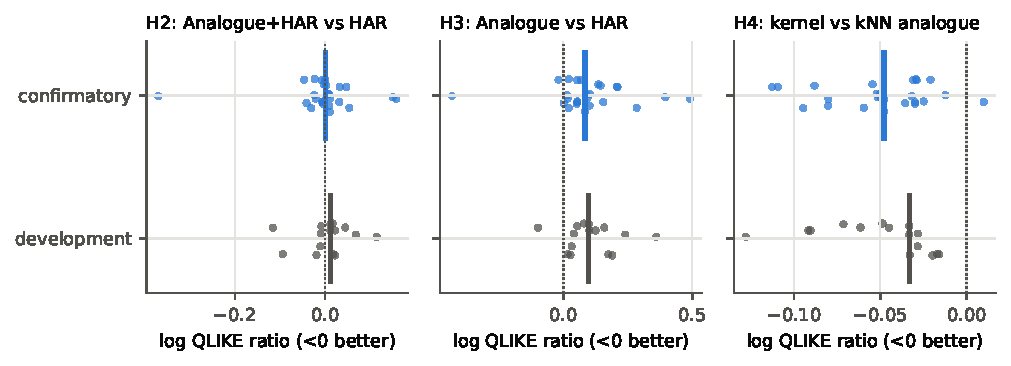
\includegraphics[width=\linewidth]{fig_hypotheses.pdf}
\caption{Per-series log QLIKE ratios for H2--H4 (points) and their medians (bars). Negative values
favour the first-named model.}
\label{fig:hyp}
\end{figure}

\subsection{Direction: no predictability}
Table~\ref{tab:direction} reports the information coefficient (IC; Spearman correlation between
the forecast and the realised R-multiple of the trade), the Brier skill of the direction
probability, and out-of-sample Sharpe ratios. Across 24 assets the IC never exceeds 0.06 in
absolute value, the mean IC is \dirMeanICDev\ in the development set and \dirMeanICCon\ in the
confirmatory set, and H1 is confirmed ($p=0.60$). Richer embeddings ($m=4$) do not help. The
bar-for-bar replication of the original strategy (v1) and the walk-forward-selected v2 both trail
buy-and-hold on almost every asset with positive drift, and the best deflated Sharpe ratio over
the 18-configuration grid is \dirMaxDSRDev\ (development) and \dirMaxDSRCon\ (confirmatory), far below
the 0.95 needed to claim skill. Positive Brier skill appears only for Nasdaq-100 and gold (development) and oil (confirmatory);
all three had large changes in drift between the calibration and out-of-sample periods, which a
fixed climatological benchmark cannot track, and none has a significant IC.

The original system's claim that aggregating to higher frequencies acts as a ``low-pass filter''
receives only weak support: for Bitcoin the IC rises from 0.004 (15-minute bars) to 0.006
(hourly) and 0.02--0.035 (4-hour), but the 4-hour sample contains roughly a thousand independent
20-bar outcomes, and an IC of 0.03 is within sampling error.

\begin{table}[t]
\centering\scriptsize
\caption{Direction. IC: out-of-sample Spearman correlation between the analogue forecast and the
realised trade R-multiple. Sharpe ratios at 5\,bp per side. DSR: deflated Sharpe ratio of the
walk-forward-selected v2 over its 18-configuration grid.}
\label{tab:direction}
\resizebox{\linewidth}{!}{\begin{tabular}{lrrrrrrr}
\toprule
& \multicolumn{2}{c}{IC (long)} & Brier & \multicolumn{3}{c}{Sharpe ratio} & \\
\cmidrule(lr){2-3}\cmidrule(lr){5-7}
Asset & $m{=}1$ & $m{=}4$ & skill & B\&H & v1 & v2 WF & DSR \\
\midrule
\multicolumn{8}{l}{\textit{Development set}}\\
BTC & 0.006 & 0.028 & -0.028 & 0.84 & -0.44 & -0.12 & 0.01\\
ETH & 0.006 & 0.014 & -0.029 & 0.78 & -1.04 & -0.76 & 0.00\\
EUR/USD & -0.014 & -0.027 & -0.025 & -0.15 & -0.35 & -0.43 & 0.00\\
Gold & -0.040 & 0.012 & 0.077 & 0.71 & 0.34 & 0.40 & 0.42\\
NIFTY 50 & -0.058 & -0.030 & -0.051 & 0.62 & -0.00 & -0.64 & 0.00\\
Nasdaq-100 & -0.032 & -0.027 & 0.025 & 0.96 & 0.25 & 0.44 & 0.58\\
PAXG & -0.007 & 0.005 & -0.030 & 0.95 & -0.85 & -1.14 & 0.00\\
S\&P 500 & -0.006 & 0.005 & -0.057 & 0.55 & 0.10 & 0.08 & 0.32\\
Treasuries & 0.019 & -0.018 & -0.029 & -0.16 & 0.03 & -0.29 & 0.00\\
\midrule
\multicolumn{8}{l}{\textit{Confirmatory set}}\\
ADA & 0.011 & 0.018 & -0.031 & 0.67 & -0.51 & -0.43 & 0.00\\
BNB & -0.001 & 0.014 & -0.027 & 1.13 & -0.65 & -0.06 & 0.01\\
DAX & 0.002 & -0.007 & -0.047 & 0.37 & 0.17 & -0.12 & 0.01\\
Emerging mkts & 0.006 & -0.024 & -0.053 & 0.30 & -0.51 & -0.12 & 0.04\\
FTSE 100 & -0.001 & 0.021 & -0.068 & 0.27 & 0.14 & -0.05 & 0.01\\
GBP/USD & 0.013 & -0.023 & -0.026 & -0.12 & 0.21 & -0.08 & 0.06\\
Hang Seng & 0.005 & 0.001 & -0.078 & 0.25 & 0.12 & 0.02 & 0.06\\
LTC & 0.001 & 0.009 & -0.032 & 0.46 & -1.28 & -0.44 & 0.00\\
Nikkei 225 & 0.009 & 0.035 & -0.047 & 0.32 & 0.11 & -0.02 & 0.03\\
Oil & -0.034 & -0.052 & 0.113 & 0.34 & 0.03 & -0.11 & 0.02\\
Russell 2000 & -0.007 & 0.016 & -0.052 & 0.52 & -0.42 & 0.00 & 0.06\\
SOL & -0.010 & -0.001 & -0.037 & 0.82 & -1.33 & -0.92 & 0.00\\
Silver & 0.006 & -0.002 & -0.048 & 0.49 & -0.20 & -0.74 & 0.00\\
USD/JPY & -0.007 & 0.017 & -0.040 & 0.18 & -0.02 & -0.20 & 0.01\\
XRP & 0.004 & 0.027 & -0.028 & 0.81 & -0.95 & 0.66 & 0.46\\
\bottomrule
\end{tabular}
}
\end{table}

\subsection{Volatility: competitive in combination}
Table~\ref{tab:volsum} summarises 40 series--horizon pairs (full results in
Appendix~\ref{app:vol}). The analogue forecaster alone is 11\% worse than HAR on average and
significantly worse (H3). Combined with HAR it is statistically indistinguishable from HAR (H2;
median ratio 1.001 in the confirmatory set) and remains in the 90\% model confidence set in 23 of
25 confirmatory series, compared with 24 for HAR and 20 for GARCH(1,1); these two counts are
unchanged when bootstrap block lengths are chosen automatically (Appendix~\ref{app:rob}). This
replicates, prospectively and across asset classes, the finding of \citet{andrada2016} for the
S\&P 100: combining nearest-neighbour and model-based forecasts does not reliably improve
statistical accuracy. Gradient-boosted trees
given a superset of the same information are the worst model, with median QLIKE 42--52\% above
HAR, and are in the confidence set for 2 of 40 series (H5): with a few thousand effectively independent observations
the flexible model overfits the noisy volatility proxy, while the analogue estimator's
averaging over whole outcome windows limits its variance.

\begin{table}[t]
\centering\scriptsize
\caption{Volatility forecasting summary (QLIKE relative to HAR; lower is better).}
\label{tab:volsum}
\resizebox{\linewidth}{!}{\begin{tabular}{lrrrrrr}
\toprule
& EWMA & GARCH & HAR & GBM & Analogue & Analogue+HAR \\
\midrule
\multicolumn{7}{l}{\textit{Development set (15 series)}}\\
Mean QLIKE / HAR & 1.063 & 1.006 & 1.000 & 1.541 & 1.119 & 1.007\\
Median QLIKE / HAR & 1.049 & 1.003 & 1.000 & 1.522 & 1.103 & 1.012\\
In 90\% MCS & 11 & 14 & 14 & 0 & 8 & 14\\
Lowest QLIKE & 0 & 7 & 4 & 0 & 0 & 4\\
\midrule
\multicolumn{7}{l}{\textit{Confirmatory set (25 series)}}\\
Mean QLIKE / HAR & 1.077 & 1.007 & 1.000 & 1.566 & 1.115 & 1.002\\
Median QLIKE / HAR & 1.051 & 0.986 & 1.000 & 1.423 & 1.087 & 1.001\\
In 90\% MCS & 18 & 20 & 24 & 2 & 12 & 23\\
Lowest QLIKE & 1 & 14 & 2 & 0 & 1 & 7\\
\bottomrule
\end{tabular}
}
\end{table}

Figure~\ref{fig:cum} shows that the combination's advantage over HAR is not driven by a few
episodes: on Bitcoin the cumulative QLIKE gain rises steadily from 2024, while on the S\&P 500 the
combination is ahead of HAR for most of seven decades but loses ground in the 1987 and 2020 crashes. GARCH loses heavily to HAR on Bitcoin but leads on the S\&P
500, in line with the view that no single volatility model dominates \citep{hansen2005}.

\begin{figure}[t]
\centering
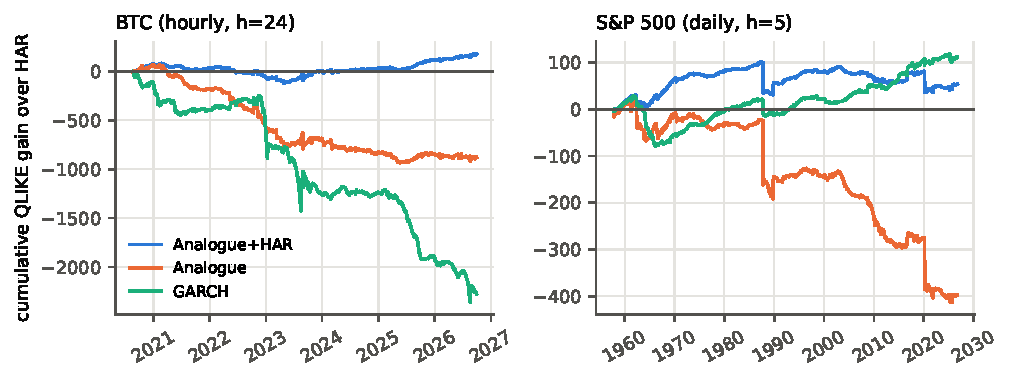
\includegraphics[width=\linewidth]{fig_cumulative_loss.pdf}
\caption{Cumulative QLIKE gain over HAR (development set). Rising lines beat HAR.}
\label{fig:cum}
\end{figure}

\paragraph{Ablations} Table~\ref{tab:abl} varies one design element at a time. The exclusion zone
and the full history each improve QLIKE by 2--3\%, confirming that independent outcomes and
many candidates matter. The Markov regime mixture has no measurable effect. The Gaussian kernel is
5\% better than $k$NN in both sets; this was found after the development protocol was fixed,
registered as H4, and confirmed ($p<10^{-6}$). Kernel weighting is therefore the recommended
default for future work.

\begin{table}[t]
\centering\scriptsize
\caption{Ablations: mean QLIKE relative to the full $k$NN analogue model ($<1$: the variant is
better).}
\label{tab:abl}
\resizebox{\linewidth}{!}{\begin{tabular}{lrrrrrrr}
\toprule
& \rotatebox{60}{m=1 (level only)} & \rotatebox{60}{m=2} & \rotatebox{60}{m=8} & \rotatebox{60}{no regime mixture} & \rotatebox{60}{no exclusion zone} & \rotatebox{60}{Gaussian kernel (bw 0.6)} & \rotatebox{60}{history capped at 5000}\\
\midrule
Development & 0.994 & 0.984 & 1.007 & 1.007 & 1.021 & 0.952 & 1.020\\
Confirmatory & 0.990 & 0.980 & 1.022 & 0.990 & 1.030 & 0.952 & 1.023\\
\bottomrule
\end{tabular}
}
\end{table}

\subsection{Tail events: clustering is volatility}
Table~\ref{tab:tail} evaluates forecasts of at least one raw jump in the next $h$ bars. The static
Poisson rule of the original system is \emph{worse than a constant forecast} in 11 of 15
development and 20 of 25 confirmatory series: a 1,000-bar average of past jump counts lags turning
points in risk. A Hawkes process fixes this (H6; median log-loss ratio 0.85 versus Poisson), but a
one-variable logistic regression on the EWMA variance is better still, with the lowest log-loss in
most series. Jump clustering is therefore largely volatility clustering, and a Hawkes intensity
adds little once the current variance is known. Figure~\ref{fig:rel} shows that the Poisson rule is
also miscalibrated: its highest-risk bin has a lower realised jump frequency than its middle bins.

\begin{table}[t]
\centering\scriptsize
\caption{Jump forecasts: probability of at least one raw jump ($|r|>3\bar\sigma$) in the next $h$ bars.}
\label{tab:tail}
\resizebox{\linewidth}{!}{\begin{tabular}{lrrrrr}
\toprule
& Constant & Poisson (v1) & Hawkes & Logistic-EWMA & Analogue \\
\midrule
\multicolumn{6}{l}{\textit{Development set}}\\
Mean log-loss / constant & 1.000 & 1.034 & 0.944 & 0.904 & 0.926\\
Mean AUC & 0.432 & 0.490 & 0.570 & 0.670 & 0.656\\
Best log-loss (series) & 0 & 0 & 0 & 12 & 3\\
Worse than constant & 0 & 11 & 1 & 0 & 2\\
\midrule
\multicolumn{6}{l}{\textit{Confirmatory set}}\\
Mean log-loss / constant & 1.000 & 1.061 & 0.901 & 0.893 & 0.911\\
Mean AUC & 0.437 & 0.502 & 0.613 & 0.710 & 0.679\\
Best log-loss (series) & 0 & 1 & 6 & 16 & 2\\
Worse than constant & 0 & 20 & 0 & 1 & 2\\
\bottomrule
\end{tabular}
}
\end{table}

\begin{figure}[t]
\centering
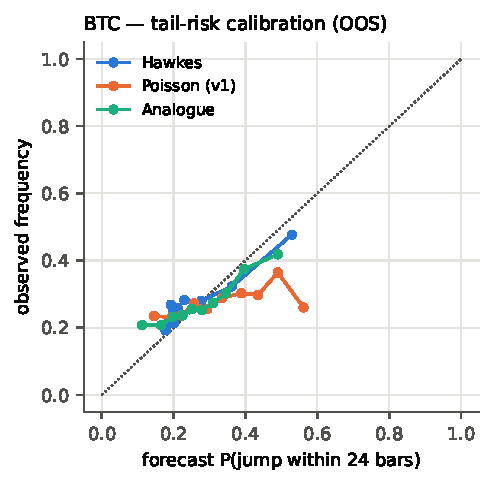
\includegraphics[width=0.5\linewidth]{fig_tail_reliability.pdf}
\caption{Reliability of jump-probability forecasts for Bitcoin (out-of-sample deciles).}
\label{fig:rel}
\end{figure}

\subsection{Value-at-Risk and Expected Shortfall: calibrated but not sharper}
Table~\ref{tab:var} compares one-day VaR/ES forecasts at 1\%, 2.5\% and 5\%. Historical simulation
and Gaussian GARCH fail coverage tests most often. The analogue-conditioned residual distribution
passes the Kupiec test as often as FHS (69\% of confirmatory cases for both) but ranks lower on the
FZ0 loss: 250 analogues per regime give a noisier estimate of a 1\% quantile than the full residual
history. Averaging the two (Blend) recovers FHS-level accuracy but does not improve on it (H7),
and FHS, Blend and GARCH-$t$ form the top group in both sets.

\begin{table}[t]
\centering\scriptsize
\caption{One-day VaR/ES. Pass rates are the share of series $\times$ $\alpha$ cases with $p>0.05$.}
\label{tab:var}
\resizebox{\linewidth}{!}{\begin{tabular}{lrrrrrr}
\toprule
& HS & GARCH-N & GARCH-t & FHS & Analogue & Blend \\
\midrule
\multicolumn{7}{l}{\textit{Development set}}\\
Mean $|$hit rate$/\alpha - 1|$ & 0.231 & 0.267 & 0.164 & 0.162 & 0.144 & 0.144\\
Kupiec pass rate & 0.63 & 0.59 & 0.78 & 0.85 & 0.89 & 0.89\\
Christoffersen CC pass rate & 0.41 & 0.56 & 0.67 & 0.74 & 0.81 & 0.74\\
Mean FZ0 rank (1 = best) & 5.81 & 3.85 & 1.89 & 2.30 & 4.74 & 2.41\\
In 90\% MCS (FZ0) & 0.52 & 0.85 & 1.00 & 1.00 & 0.63 & 1.00\\
\midrule
\multicolumn{7}{l}{\textit{Confirmatory set}}\\
Mean $|$hit rate$/\alpha - 1|$ & 0.243 & 0.338 & 0.228 & 0.176 & 0.184 & 0.162\\
Kupiec pass rate & 0.51 & 0.42 & 0.58 & 0.69 & 0.69 & 0.67\\
Christoffersen CC pass rate & 0.31 & 0.44 & 0.60 & 0.71 & 0.67 & 0.71\\
Mean FZ0 rank (1 = best) & 5.47 & 4.07 & 2.36 & 2.31 & 4.47 & 2.33\\
In 90\% MCS (FZ0) & 0.40 & 0.71 & 0.87 & 1.00 & 0.73 & 0.98\\
\bottomrule
\end{tabular}
}
\end{table}

\subsection{Economic value: lower drawdowns, not higher Sharpe ratios}
Scaling a long position by the Analogue+HAR volatility forecast reduced the maximum drawdown for
all 9 development and all 15 confirmatory assets (H8; median reduction 5.6 percentage points in the
confirmatory set) at the cost of slightly lower Sharpe ratios (median change $-0.015$; positive for
5 of 15 assets). This is the pattern documented by \citet{cederburg2020}: volatility management
reliably reduces risk but does not reliably improve risk-adjusted returns out of sample. With
dividend-adjusted prices for the four distribution-paying funds, Sharpe ratio levels rise but every
comparison keeps its sign (Appendix~\ref{app:rob}). The
Hawkes ``lock-out'' of the original system lowered the Sharpe ratio further for 9 of 15
confirmatory assets, and significantly so for Bitcoin and Ethereum in the development set, because the periods after
jumps include sharp rebounds (Table~\ref{tab:overlay}, Figure~\ref{fig:eq}).

\begin{table}[t]
\centering\scriptsize
\caption{Volatility-managed long exposure (no leverage, 5\,bp per unit turnover). $p$: paired
stationary-bootstrap test of the Sharpe difference with buy-and-hold.}
\label{tab:overlay}
\resizebox{\linewidth}{!}{\begin{tabular}{lrrrrrr}
\toprule
& \multicolumn{4}{c}{Sharpe ratio} & \multicolumn{2}{c}{Max drawdown (\%)} \\
\cmidrule(lr){2-5}\cmidrule(lr){6-7}
Asset & B\&H & Vol target & $p$ & + Hawkes gate & B\&H & Vol target \\
\midrule
\multicolumn{7}{l}{\textit{Development set}}\\
BTC & 0.84 & 0.78 & 0.30 & 0.34 & -77.2 & -75.9\\
ETH & 0.78 & 0.71 & 0.39 & 0.34 & -81.3 & -76.0\\
EUR/USD & -0.11 & -0.10 & 0.30 & -0.15 & -35.4 & -35.3\\
Gold & 0.44 & 0.47 & 0.32 & 0.47 & -45.6 & -42.7\\
NIFTY 50 & 0.72 & 0.72 & 0.83 & 0.72 & -38.4 & -31.2\\
Nasdaq-100 & 0.75 & 0.84 & 0.13 & 0.84 & -53.6 & -41.6\\
PAXG & 0.95 & 1.35 & 0.02 & 0.90 & -29.2 & -21.2\\
S\&P 500 & 0.55 & 0.58 & 0.19 & 0.60 & -56.8 & -49.3\\
Treasuries & -0.00 & -0.05 & 0.15 & -0.03 & -54.2 & -53.8\\
\midrule
\multicolumn{7}{l}{\textit{Confirmatory set}}\\
ADA & 0.67 & 0.42 & 0.00 & -0.23 & -95.5 & -95.0\\
BNB & 1.13 & 1.08 & 0.58 & 0.67 & -72.5 & -70.9\\
DAX & 0.37 & 0.38 & 0.86 & 0.41 & -72.7 & -62.7\\
Emerging mkts & 0.23 & 0.23 & 0.11 & 0.13 & -43.7 & -43.7\\
FTSE 100 & 0.27 & 0.22 & 0.25 & -0.01 & -52.6 & -46.6\\
GBP/USD & -0.09 & -0.10 & 0.31 & -0.05 & -37.5 & -37.4\\
Hang Seng & 0.25 & 0.23 & 0.63 & 0.10 & -65.2 & -58.3\\
LTC & 0.46 & 0.42 & 0.52 & 0.17 & -90.4 & -85.2\\
Nikkei 225 & 0.32 & 0.32 & 1.00 & 0.23 & -81.9 & -70.1\\
Oil & 0.09 & 0.08 & 0.85 & 0.08 & -94.6 & -85.2\\
Russell 2000 & 0.43 & 0.39 & 0.53 & 0.39 & -54.9 & -37.5\\
SOL & 0.82 & 0.83 & 0.93 & 0.19 & -82.7 & -77.2\\
Silver & 0.33 & 0.34 & 0.86 & 0.34 & -67.0 & -66.7\\
USD/JPY & 0.19 & 0.22 & 0.50 & 0.22 & -38.8 & -33.7\\
XRP & 0.81 & 0.60 & 0.10 & 0.22 & -84.8 & -75.1\\
\bottomrule
\end{tabular}
}
\end{table}

\begin{figure}[t]
\centering
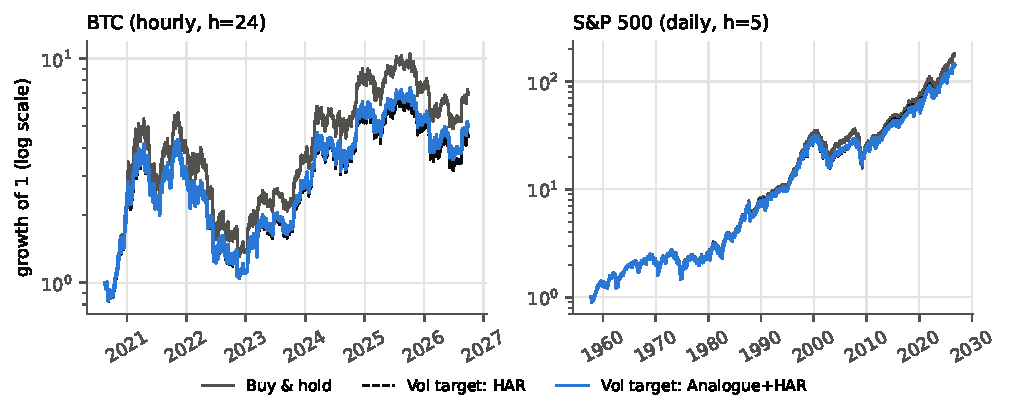
\includegraphics[width=\linewidth]{fig_overlay_equity.pdf}
\caption{Growth of one unit, out-of-sample (development set).}
\label{fig:eq}
\end{figure}

\subsection{Interpretability and computation}
Every analogue forecast can be decomposed into its analogues. Figure~\ref{fig:explain} shows the
hour of the FTX collapse in November 2022: the ten nearest historical volatility shapes, what
followed them, and the forecast. Here the analogues predicted a partial reversion of volatility
that did not occur, which is the kind of error a user can see and reason about. The engine
forecasts about 30,000 bars per second with a capped history and 200,000 bars in about 90 seconds
with the full-history search on a 10-core laptop; the complete confirmatory study ran in under
half an hour.

\begin{figure}[t]
\centering
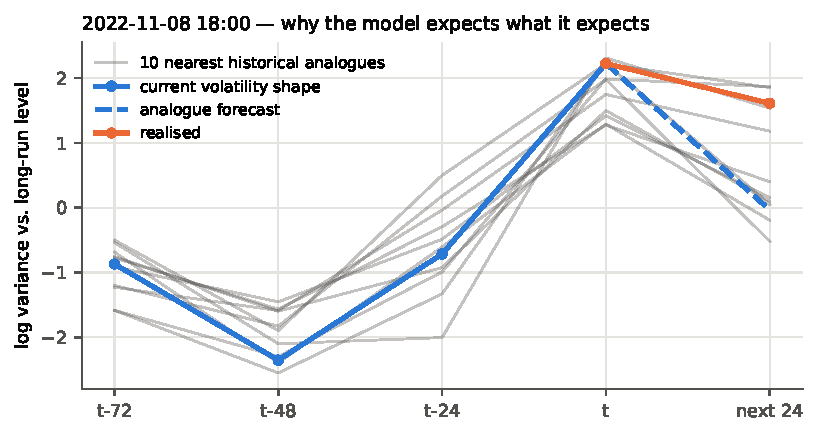
\includegraphics[width=\linewidth]{fig_analogue_explanation.pdf}
\caption{A forecast and its analogues: BTC, 8 November 2022, 18:00 UTC.}
\label{fig:explain}
\end{figure}

%% ==================================================================
\section{Discussion}

\paragraph{Where the predictability is} The analogue engine extracts no information about the
direction of prices but a substantial amount about their risk. This mirrors the broader
distinction between the unpredictability of returns \citep{fama1970} and the strong predictability
of volatility \citep{bollerslev1986,corsi2009}, and it holds across cryptocurrencies, equity
indices, commodities, bonds and currencies, at hourly and daily frequency.

\paragraph{Implications for the original system} Of the original system's components, the
directional analogue signal and the Poisson crash gate do not survive out-of-sample testing: the
former has no skill, and the latter is worse than a constant. The regime mixture, which replaced
an ad hoc adjustment, is harmless but adds nothing measurable. What survives is the core idea of
matching the present to the past, redirected from direction to risk, where it is competitive with
the standard models and yields well-calibrated tail forecasts with a transparent justification.

\paragraph{Why pre-registration mattered} Two development findings could have been overstated
without the confirmatory test. The analogue VaR was the best-calibrated model in development but
only tied with FHS on new assets; the kernel variant, found after the development design was
fixed, might have been dismissed as a lucky ablation but replicated with $p<10^{-6}$.
Pre-registration separated these cases at negligible cost.

\paragraph{Limitations} Realised variance is computed from bar returns rather than intraday
data, which adds noise to the target for daily series. The Analogue+HAR combination uses fixed
equal weights. The embedding uses only a single series; cross-asset analogues are a natural
extension. Transaction-cost assumptions are stylised, and the overlay ignores financing and cash
returns. The main tables use unadjusted closing prices, as registered; Appendix~\ref{app:rob} shows
that dividend adjustment does not change the conclusions.

%% ==================================================================
\section{Conclusion}
A pre-registered evaluation on 24 assets shows that analogue forecasting, a popular and
interpretable tool, has no directional value in financial markets but produces risk forecasts
that are competitive with HAR and GARCH, calibrated tail forecasts, and reliable drawdown
reductions. Its most useful design elements are an exclusion zone that keeps analogues
independent, the full history, and kernel weighting. We release the engine and the
pre-registration so that other analogue methods can be tested the same way.

\appendix
\section{Full volatility results}
\label{app:vol}
Bold entries are in the 90\% model confidence set.
\begin{center}\resizebox{0.9\linewidth}{!}{\begin{tabular}{lrrrrrr}
\toprule
Series (horizon) & EWMA & GARCH & HAR & GBM & Analogue & Analogue+HAR \\
\midrule
\multicolumn{7}{l}{\textit{Development set}}\\
BTC (h=24) & 1.101 & 1.107 & \textbf{1.000} & 1.270 & 1.041 & \textbf{0.992}\\
ETH (h=24) & 1.147 & \textbf{1.067} & \textbf{1.000} & 1.251 & \textbf{1.033} & \textbf{0.990}\\
EUR/USD (h=22) & \textbf{0.987} & \textbf{1.078} & \textbf{1.000} & 1.399 & \textbf{1.017} & \textbf{0.911}\\
EUR/USD (h=5) & \textbf{0.939} & \textbf{0.928} & 1.000 & 1.525 & 1.028 & 0.982\\
Gold (h=22) & \textbf{0.896} & \textbf{1.003} & \textbf{1.000} & 1.527 & \textbf{0.906} & \textbf{0.891}\\
Gold (h=5) & \textbf{1.015} & \textbf{0.969} & \textbf{1.000} & 1.625 & \textbf{1.103} & \textbf{1.012}\\
NIFTY 50 (h=22) & \textbf{1.044} & \textbf{0.894} & \textbf{1.000} & 2.016 & \textbf{1.272} & \textbf{1.071}\\
NIFTY 50 (h=5) & \textbf{1.073} & \textbf{1.004} & \textbf{1.000} & 1.574 & \textbf{1.106} & \textbf{1.023}\\
Nasdaq-100 (h=22) & \textbf{1.262} & \textbf{0.980} & \textbf{1.000} & 1.974 & 1.434 & \textbf{1.122}\\
Nasdaq-100 (h=5) & \textbf{1.022} & \textbf{0.942} & \textbf{1.000} & 2.139 & 1.084 & \textbf{1.018}\\
PAXG (h=24) & \textbf{1.109} & \textbf{1.087} & \textbf{1.000} & 1.308 & \textbf{1.172} & \textbf{1.047}\\
S\&P 500 (h=22) & 1.222 & \textbf{1.023} & \textbf{1.000} & 1.466 & 1.209 & \textbf{1.023}\\
S\&P 500 (h=5) & 1.075 & \textbf{0.984} & \textbf{1.000} & 1.152 & 1.056 & \textbf{0.992}\\
Treasuries (h=22) & \textbf{1.049} & \textbf{1.042} & \textbf{1.000} & 1.522 & \textbf{1.190} & \textbf{1.019}\\
Treasuries (h=5) & \textbf{1.010} & \textbf{0.975} & \textbf{1.000} & 1.368 & 1.133 & \textbf{1.012}\\
\addlinespace Mean ratio & 1.063 & 1.006 & 1.000 & 1.541 & 1.119 & 1.007\\
In 90\% MCS & 11/15 & 14/15 & 14/15 & 0/15 & 8/15 & 14/15\\
\midrule
\multicolumn{7}{l}{\textit{Confirmatory set}}\\
ADA (h=24) & 1.105 & 1.071 & \textbf{1.000} & 1.323 & \textbf{1.014} & \textbf{0.977}\\
BNB (h=24) & 1.151 & 1.162 & \textbf{1.000} & 1.242 & 1.070 & \textbf{1.001}\\
DAX (h=22) & 1.181 & \textbf{0.972} & \textbf{1.000} & 1.256 & 1.329 & 1.056\\
DAX (h=5) & 1.044 & \textbf{0.962} & 1.000 & 1.281 & 1.055 & 0.993\\
Emerging mkts (h=22) & \textbf{1.241} & \textbf{0.990} & \textbf{1.000} & \textbf{1.307} & \textbf{1.167} & \textbf{1.033}\\
Emerging mkts (h=5) & \textbf{1.051} & \textbf{0.984} & \textbf{1.000} & 1.358 & 1.098 & \textbf{1.012}\\
FTSE 100 (h=22) & \textbf{1.037} & \textbf{0.927} & \textbf{1.000} & 1.695 & 1.146 & \textbf{0.998}\\
FTSE 100 (h=5) & \textbf{0.993} & \textbf{0.936} & \textbf{1.000} & 1.410 & \textbf{1.017} & \textbf{0.980}\\
GBP/USD (h=22) & \textbf{0.983} & \textbf{0.991} & \textbf{1.000} & 1.624 & 1.108 & \textbf{1.009}\\
GBP/USD (h=5) & \textbf{1.000} & \textbf{0.982} & \textbf{1.000} & 1.645 & 1.087 & \textbf{1.011}\\
Hang Seng (h=22) & \textbf{1.017} & \textbf{0.950} & \textbf{1.000} & 1.756 & 1.231 & \textbf{1.034}\\
Hang Seng (h=5) & \textbf{1.011} & \textbf{0.986} & \textbf{1.000} & 1.423 & 1.091 & \textbf{1.008}\\
LTC (h=24) & 1.114 & 1.106 & \textbf{1.000} & 1.330 & 1.055 & \textbf{0.997}\\
Nikkei 225 (h=22) & \textbf{1.125} & \textbf{1.130} & \textbf{1.000} & 1.598 & \textbf{1.155} & \textbf{1.003}\\
Nikkei 225 (h=5) & 1.118 & 1.078 & \textbf{1.000} & 1.348 & 1.056 & \textbf{0.994}\\
Oil (h=22) & \textbf{1.362} & \textbf{0.986} & \textbf{1.000} & \textbf{2.214} & \textbf{1.486} & \textbf{1.164}\\
Oil (h=5) & \textbf{1.081} & \textbf{1.061} & \textbf{1.000} & 1.889 & \textbf{1.021} & \textbf{0.971}\\
Russell 2000 (h=22) & \textbf{1.333} & \textbf{0.924} & \textbf{1.000} & 1.808 & \textbf{1.634} & \textbf{1.172}\\
Russell 2000 (h=5) & \textbf{1.011} & \textbf{0.946} & \textbf{1.000} & 1.959 & 1.107 & \textbf{1.010}\\
SOL (h=24) & 1.105 & 1.110 & \textbf{1.000} & 1.313 & 1.053 & \textbf{0.996}\\
Silver (h=22) & \textbf{0.976} & \textbf{0.927} & \textbf{1.000} & 2.720 & \textbf{1.234} & \textbf{1.049}\\
Silver (h=5) & \textbf{0.979} & \textbf{0.970} & \textbf{1.000} & 1.600 & \textbf{1.002} & \textbf{0.960}\\
USD/JPY (h=22) & \textbf{0.658} & \textbf{1.058} & \textbf{1.000} & 1.432 & \textbf{0.650} & \textbf{0.691}\\
USD/JPY (h=5) & \textbf{1.012} & \textbf{0.977} & \textbf{1.000} & 1.375 & \textbf{1.021} & \textbf{0.978}\\
XRP (h=24) & \textbf{1.235} & \textbf{1.000} & \textbf{1.000} & 1.249 & \textbf{0.982} & \textbf{0.955}\\
\addlinespace Mean ratio & 1.077 & 1.007 & 1.000 & 1.566 & 1.115 & 1.002\\
In 90\% MCS & 18/25 & 20/25 & 24/25 & 2/25 & 12/25 & 23/25\\
\bottomrule
\end{tabular}
}\end{center}

\section{Robustness}
\label{app:rob}

\paragraph{Dividend-adjusted prices} The study uses Yahoo's unadjusted closing prices, as
registered. Price indices (S\&P 500, DAX and the like) have no adjusted series, and the gold,
silver and oil funds pay no distributions, so adjustment matters only for the Nasdaq-100,
long-Treasury, Russell 2000 and emerging-markets funds. Re-running the volatility and overlay
experiments on their dividend-adjusted prices (Table~\ref{tab:robadj}) moves QLIKE ratios by at
most 0.026. Sharpe ratio levels rise for both buy-and-hold and volatility targeting---most for
Treasuries, where coupons are the bulk of the return---but every comparison keeps its sign:
volatility targeting still lowers the maximum drawdown and still slightly lowers the Sharpe ratio
for three of the four funds.

\begin{table}[h]
\centering\scriptsize
\caption{Unadjusted versus dividend-adjusted prices (volatility: $h=5$ and $h=22$; overlay: $h=5$).}
\label{tab:robadj}
\resizebox{\linewidth}{!}{\begin{tabular}{llrrr}
\toprule
Series & Quantity & Unadjusted & Adjusted & Change \\
\midrule
Emerging mkts (h=22) & QLIKE / HAR: Analogue+HAR & 1.033 & 1.033 & -0.000\\
Emerging mkts (h=5) & QLIKE / HAR: Analogue+HAR & 1.012 & 1.007 & -0.005\\
Nasdaq-100 (h=22) & QLIKE / HAR: Analogue+HAR & 1.122 & 1.117 & -0.005\\
Nasdaq-100 (h=5) & QLIKE / HAR: Analogue+HAR & 1.018 & 1.012 & -0.006\\
Russell 2000 (h=22) & QLIKE / HAR: Analogue+HAR & 1.172 & 1.162 & -0.010\\
Russell 2000 (h=5) & QLIKE / HAR: Analogue+HAR & 1.010 & 1.006 & -0.004\\
Treasuries (h=22) & QLIKE / HAR: Analogue+HAR & 1.019 & 1.026 & +0.007\\
Treasuries (h=5) & QLIKE / HAR: Analogue+HAR & 1.012 & 1.010 & -0.002\\
Nasdaq-100 & Buy \& hold: Sharpe & 0.749 & 0.785 & +0.036\\
Nasdaq-100 & Buy \& hold: max DD & -0.536 & -0.534 & +0.001\\
Nasdaq-100 & Vol target: Analogue+HAR: Sharpe & 0.839 & 0.882 & +0.043\\
Nasdaq-100 & Vol target: Analogue+HAR: max DD & -0.416 & -0.409 & +0.007\\
Treasuries & Buy \& hold: Sharpe & -0.001 & 0.198 & +0.198\\
Treasuries & Buy \& hold: max DD & -0.542 & -0.484 & +0.058\\
Treasuries & Vol target: Analogue+HAR: Sharpe & -0.045 & 0.179 & +0.224\\
Treasuries & Vol target: Analogue+HAR: max DD & -0.538 & -0.446 & +0.092\\
Russell 2000 & Buy \& hold: Sharpe & 0.426 & 0.481 & +0.055\\
Russell 2000 & Buy \& hold: max DD & -0.549 & -0.543 & +0.006\\
Russell 2000 & Vol target: Analogue+HAR: Sharpe & 0.389 & 0.480 & +0.090\\
Russell 2000 & Vol target: Analogue+HAR: max DD & -0.375 & -0.352 & +0.023\\
Emerging mkts & Buy \& hold: Sharpe & 0.235 & 0.332 & +0.098\\
Emerging mkts & Buy \& hold: max DD & -0.437 & -0.398 & +0.039\\
Emerging mkts & Vol target: Analogue+HAR: Sharpe & 0.228 & 0.325 & +0.098\\
Emerging mkts & Vol target: Analogue+HAR: max DD & -0.437 & -0.393 & +0.045\\
\bottomrule
\end{tabular}
}
\end{table}

\paragraph{Bootstrap block lengths} Model confidence sets and Sharpe-difference tests use the
stationary bootstrap with fixed mean block lengths ($2h$; ten days for VaR/ES). Replacing them by
the automatic choice of \citet{politis2004}, with the correction of \citet{patton2009}, leaves the
headline counts unchanged---Analogue+HAR remains in the 90\% confidence set for 14 of 15
development and 23 of 25 confirmatory series, HAR for 14 and 24---and changes 19 of 672
confidence-set verdicts and 3 of 168 test verdicts (Table~\ref{tab:robblk}). The automatic lengths
are slightly more conservative, so the changes mostly admit additional models to a confidence set.

\begin{table}[h]
\centering\scriptsize
\caption{Fixed versus Politis--White bootstrap block lengths.}
\label{tab:robblk}
\resizebox{\linewidth}{!}{\begin{tabular}{llrlrrr}
\toprule
Set & Test & Cases & Verdict & Fixed & Politis--White & Changed \\
\midrule
Development & Volatility MCS (e2) & 90 & in MCS & 61 & 61 & 0\\
Development & VaR/ES MCS (e8) & 162 & in MCS & 135 & 135 & 2\\
Development & Overlay Sharpe test (e5) & 63 & significant & 4 & 4 & 0\\
Confirmatory & Volatility MCS (e2) & 150 & in MCS & 99 & 105 & 6\\
Confirmatory & VaR/ES MCS (e8) & 270 & in MCS & 211 & 220 & 11\\
Confirmatory & Overlay Sharpe test (e5) & 105 & significant & 14 & 13 & 3\\
\bottomrule
\end{tabular}
}
\end{table}

\paragraph{Kernel effective sample size} In kernel mode all anchors receive weight, and anchors
whose outcome windows overlap are not independent, so the \citet{kish1965} effective sample size
counted per anchor overstates the information in the analogue set. This affects the standard
error of the kernel forecast and its minimum-sample rule, not its mean, so H4, which compares
forecast accuracy, is unaffected. The released code offers an overlap-aware effective sample size
that counts each block of $h$ anchors as one observation; it is recommended for new work.



\section*{Data and code availability}
All code, the pre-registration and every result table are available at
\url{https://github.com/ManasDasri/analogue-risk} under the MIT license. The pre-registration is the
tagged commit \texttt{prereg-v1}. Price data are downloaded from public Binance and Yahoo Finance
endpoints by the included scripts.

\section*{Declaration of competing interest}
The authors hold a patent on the original trading method evaluated in this paper. The evaluation
was pre-registered and its results are reported in full.

\section*{Declaration of generative AI and AI-assisted technologies in the writing process}
During the preparation of this work the authors used Claude (Anthropic) to assist with software
development, analysis and drafting. After using this tool, the authors reviewed and edited the
content as needed and take full responsibility for the content of the publication.

\bibliographystyle{elsarticle-harv}
\bibliography{../refs}

\end{document}
